\documentclass[t]{beamer} % [t] pomeni poravnavo na vrh slida

% \usepackage{etex} % vključi ta paket, če ti javi napako, da imaš naloženih preveč paketov.

% standardni paketi
\usepackage[slovene]{babel}
\usepackage[T1]{fontenc}
\usepackage[utf8]{inputenc}
\usepackage{amssymb}
\usepackage{amsmath}
\usefonttheme[onlymath]{serif}

% paket, ki ga rabimo za risanje
\usepackage{tikz}

\usepackage{lmodern}                            % to get rid of font warnings
\renewcommand\textbullet{\ensuremath{\bullet}}  % to get rid of font warnings

% podatki
\title{Elastomehanika in numerično reševanje problemov z brezmrežnimi metodami}
\author{Jure Slak}
\institute{mentor: doc. dr. George Mejak \\
           somentor: dr. Gregor Kosec, IJS}

% tvoj izbran stil predstavitve
\usetheme{Singapore}
\usecolortheme{crane}

% \setbeamertemplate{footline}{}            % pri nekaterih temah je potrebno odstraniti
% \setbeamertemplate{navigation symbols}{}  % nogo, v tem primeru to odkomentiraj

\newcommand{\ddt}[1]{\frac{d#1}{dt}}
\newcommand{\dpar}[2]{\frac{\partial #1}{\partial #2}}
\renewcommand{\div}{\operatorname{div}}
\DeclareMathOperator{\grad}{grad}
\newcommand{\lap}{\triangle}

\newcommand{\T}{\mathsf{T}}
\renewcommand{\L}{\mathcal{L}}
\newcommand{\eps}{\varepsilon}

\usepackage[makeroom]{cancel}

%\usepackage{movie15}

\setbeamertemplate{headline}{}

%  ukaz za počrnitev enega slida. Nariše črn pravokotnik višine #1 na dno.
\newcommand{\fillblack}[1]{
\begin{tikzpicture}[remember picture, overlay]
    \node [shift={(0 cm,0cm)}]  at (current page.south west)
        {%
        \begin{tikzpicture}[remember picture, overlay] at (current page.south west)
            \draw [fill=black] (0, 0) -- (0,#1 \paperheight) --
                              (\paperwidth,#1 \paperheight) -- (\paperwidth,0) -- cycle ;
        \end{tikzpicture}
        };
        \draw (current page.north west) rectangle (current page.south east);
\end{tikzpicture}
}

\begin{document}

\begin{frame}
  \vspace{-50px}
  \maketitle
  \fillblack{0.5}
\end{frame}

\begin{frame}{Opis gibanja}
  \vspace{-4ex}
  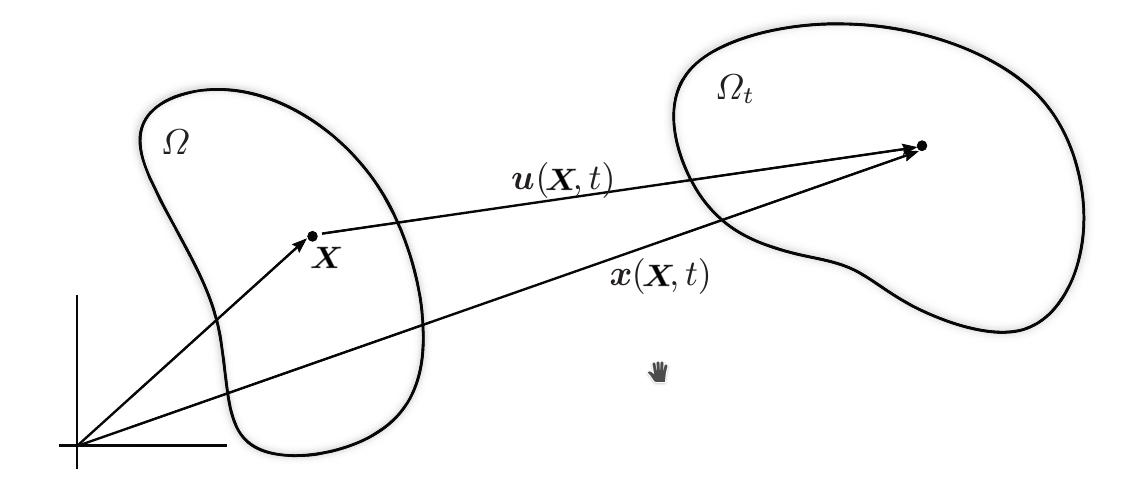
\includegraphics[width=0.9\textwidth]{movement.png}
  \fillblack{0.5}
\end{frame}

\begin{frame}{Opis gibanja -- primer}
  \begin{columns}
    \begin{column}{0.5\textwidth}
%      \vspace{-19ex}
        \href{../demos/demo_motion.nb}{
             \[ x(X, Y, t) =
        \begin{bmatrix}
          X \\ Y-1+\frac{t}{2}(Y^2-1)
        \end{bmatrix} \]}
    \end{column}
    \begin{column}{0.5\textwidth}
      \vspace{-4ex}
      \includegraphics[width=0.5\textwidth]{../demos/start.pdf}
      \includegraphics[width=0.5\textwidth]{../demos/end.pdf}
    \end{column}
  \end{columns}
%  \includemovie{5cm}{5cm}{../demos/motion.gif}
  \fillblack{0.5}
\end{frame}

\begin{frame}{Aksiomi}
%    $x$ difeomorfizem z $|\dpar{x}{X}| > 0$, $m \ll V$, $\ddt{} \int_B dm  = 0$
  \begin{align*}
    \ddt{} \int_B \dot{x} dm &= \int_B \vec{f} dV + \int_{\partial B} \vec{t} dS
    \\
    \ddt{} \int_B \dot{x} \times x dm &= \int_B \vec{f} \times x dV +
    \int_{\partial B} \vec{t} \times x dS
  \end{align*}
  \fillblack{0.5}
\end{frame}

\begin{frame}{Konstitutivne enačbe}
  Gibalna enačba:
  $ \rho \ddot{u} = \div \sigma + \vec{f} $ \\[2ex]
  \fillblack{0.5}
\end{frame}

\begin{frame}{Konstitutivne enačbe}
  Deformacija: $\eps = \frac12\left( \grad u + \grad u^\T + \cancel{\grad u \grad u^\T} \right)$ \\[2ex]
  Gibalna enačba:
  $ \rho \ddot{u} = \div \sigma + \vec{f} $ \\[2ex]
  \fillblack{0.5}
\end{frame}

\begin{frame}{Konstitutivne enačbe}
  Deformacija: $\eps = \frac12\left( \grad u + \grad u^\T \right)$ \\[2ex]
  Gibalna enačba:
  $ \rho \ddot{u} = \div \sigma + \vec{f} $ \\[2ex]
  Hookov zakon: $\sigma = C \eps$
  \fillblack{0.5}
\end{frame}

\begin{frame}{Konstitutivne enačbe}
  \vspace{-4ex}
  \begin{align*}
  &\text{Deformacija: } \eps = \frac12\left( \grad u + \grad u^\T \right) & \eps &= u' \\[2ex]
  &\text{Hookov zakon: } \sigma = C \eps
  & \sigma &= E \eps \\[2ex]
  &\text{Gibalna enačba:  } \rho \ddot{u} = \div \sigma + \vec{f}
  & \rho \ddot{u} &= \sigma' + \vec{f}
  \end{align*}
  \fillblack{0.5}
\end{frame}

\begin{frame}{Končna enačba}
  \vspace{-4ex}
  \[
  \rho \ddot{u} = E u'' + \vec{f}
  \]
  \vspace{2ex}
  \[
  \rho \ddot{u} = \frac{E}{2(1+\nu)} \left( \nabla^2 u + \frac{1}{1-2\nu}\nabla\left( \nabla\cdot u\right)  \right) + \vec{f}
  \]
  \centering
  robni pogoji: $u = 0$ ali $\vec{t} = 0$.
  \fillblack{0.5}
\end{frame}

\begin{frame}{Numerično reševanje}
  Brezmrežne metode

  \centering
  \includegraphics[width=0.7\textwidth]{../magisterij/images/domain.pdf}
\end{frame}

\begin{frame}{Metoda deljenih diferenc}
  Enačba: $u''(x) = f(x)$, $u(a) = A, u(b) = B$. \\[2ex]
  Diskretizacija: \[
  \frac{u_{i-1} - 2u_{i} + u_{i+1}}{h^2} = f(x_i)\]
  Sistem enačb:
  \[
   \begin{bmatrix}
  1 &  \\
  -1 & 2 & 1 \\
  & -1 & 2 & 1 \\
  & & \!\ddots & \!\ddots & \! \ddots \\
  &&& -1 & 2 & 1 \\
  &&&&&  1 &  \\
    \end{bmatrix}
    \begin{bmatrix}
    u_0 \\ u_1 \\ u_2 \\ \vdots \\ u_{N-1} \\ u_N
    \end{bmatrix}
    =
    \begin{bmatrix}
    A \\
    f(x_1) \\
    f(x_2) \\
    \vdots \\
    f(x_{N-1}) \\
    B
    \end{bmatrix}
  \]
\end{frame}

\begin{frame}{Izpeljava aproksimacij LPDO}
  Ideja: $(\L u)(x) \approx (\L \hat{u})(x)$, $\hat{u}$ interpolacijski polinom za $u$.
  Posplošimo: $\hat{u}(x) = \sum_{i=1}^m \alpha_i b_i(x)$; $b_i$ bazne funkcije.
  Zahtevamo, da interpolira v sosednih točkah $x_1, \dots, x_n$: $\hat{u}(x_i) = u(x_i)$.
  \[
  \begin{bmatrix}
  b_1(x_1) & \ldots & b_m(x_1) \\
  \vdots & \ddots & \vdots \\
  b_1(x_n) & \ldots & b_m(x_n)
  \end{bmatrix}
  \begin{bmatrix}
  \alpha_1 \\ \vdots \\ \alpha_m
  \end{bmatrix}
  =
  \begin{bmatrix}
  u_1 \\ \vdots \\ u_n
  \end{bmatrix}
  \]
  Rešimo in dobimo:
  \[
  \hat{u} = b(x)^\T B^{-1} u.
  \]
  Sedaj:
   \[ (\L u)(x) \approx (\L \hat{u})(x) = \underbrace{(\L b)(x)^\T B^{-1}}_{\varphi(x)} u \]
\end{frame}

\begin{frame}{Sistem enačb}
\[
\begin{bmatrix}
1  \\
\varphi(x_1) \\
\varphi(x_2) \\
\vdots \\
\varphi(x_{N-1}) \\
1   \\
\end{bmatrix}
\begin{bmatrix}
u_0 \\ u_1 \\ u_2 \\ \vdots \\ u_{N-1} \\ u_N
\end{bmatrix}
=
\begin{bmatrix}
A \\
f(x_1) \\
f(x_2) \\
\vdots \\
f(x_{N-1}) \\
B
\end{bmatrix}
\]

\vspace{4ex}

Razpršena matrika s približno $nN$ elementi.
\end{frame}

\begin{frame}{Sistem enačb}
  \vspace{-2ex}
  \centering
  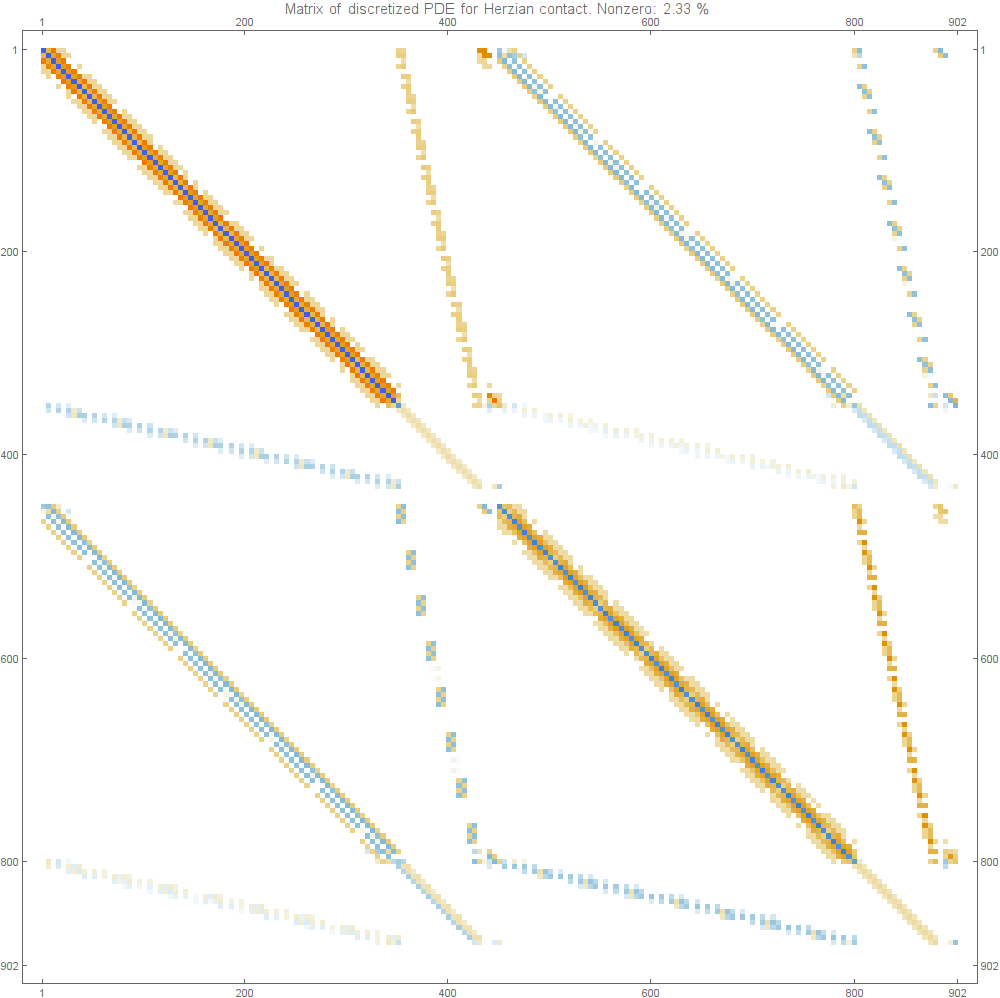
\includegraphics[width=0.8\textwidth]{Matrix_hertzian.png}
\end{frame}

\begin{frame}{Implementacija}
  \begin{enumerate}
    \item diskretizacija domene, relaksacija
    \item iskanje najbližjih sosedov (kD-tree, cover tree, ball tree)
    \item izračun ``shape funkcij'' (SVD)
    \item reševanje velikega razpršenega sistema (BiCGStab)
  \end{enumerate}
  \centering
  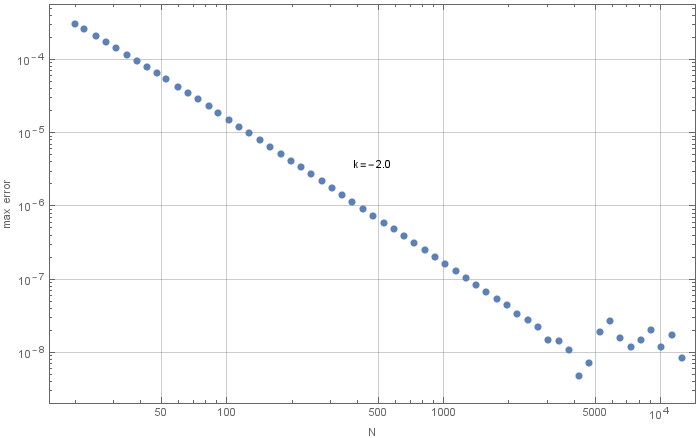
\includegraphics[width=0.7\textwidth]{MLSMerr.png}
\end{frame}



\end{document}
